\chapter{NNUE Implementierung}

Ziel dies Kapitels ist es, Architektur und Implementierung der im Rahmen dieser Arbeit entwickelten \ac{NNUE} Evaluationsfunktion zu erläutern. Es wird anfangs auf die Architekturendscheidungen eingegangen. Danach wird geklärt wie diese Entscheidungen Einfluss auf die Implementierung des Trainers und der Integration in einem Schachcomputer beeinflussen.

Kapitel \autoref{chap:HCE} zeigt wie die herkömmliche Art und Weise der Positions-Evaluation funktioniert. Verbesserungen der \ac{HCE} ist nicht einfach, jeder neue Aspekt in der Evaluationsfunktion muss sorgfältig ausgewählt werden und anschließend per Hand oder mithilfe von Optimierungsalgorithmen wie \zb{} \ac{SPSA} angepasst werden \cite{spall1992multivariate}. Es ist sehr schwer eine Evaluation zu bauen, die für alle möglichen Stellungen optimal ist. Zudem spielt der Bias der Entwickler immer eine Rolle. Die \ac{NNUE} Evaluation ist nicht an solche Limitierungen gebunden und kann auf eine ganz andere Art und Weise entscheiden welche Faktoren wichtig für die Evaluation einer Schachposition sind. Die Entwicklung der Schachcomputerlandschaft zeigt, das diese Herangehensweise der \ac{HCE} überlegen ist. Nur in Situationen, in denen es einen klaren Vorteil gibt, ist es sinnvoll \ac{HCE} zu verwenden. Deshalb verwenden die meisten \ac{NNUE} Schachcomputer einen Hybriden Ansatz, in der Implementierung dieser Arbeit wird eine reine \ac{NNUE} Evaluation verwenden. Der Grund dafür ist die rudimentäre \ac{HCE} des verwendeten Schachcomputers.


\section{Architektur}

\begin{figure}
  \centering
  \resizebox{\textwidth}{!}{%
  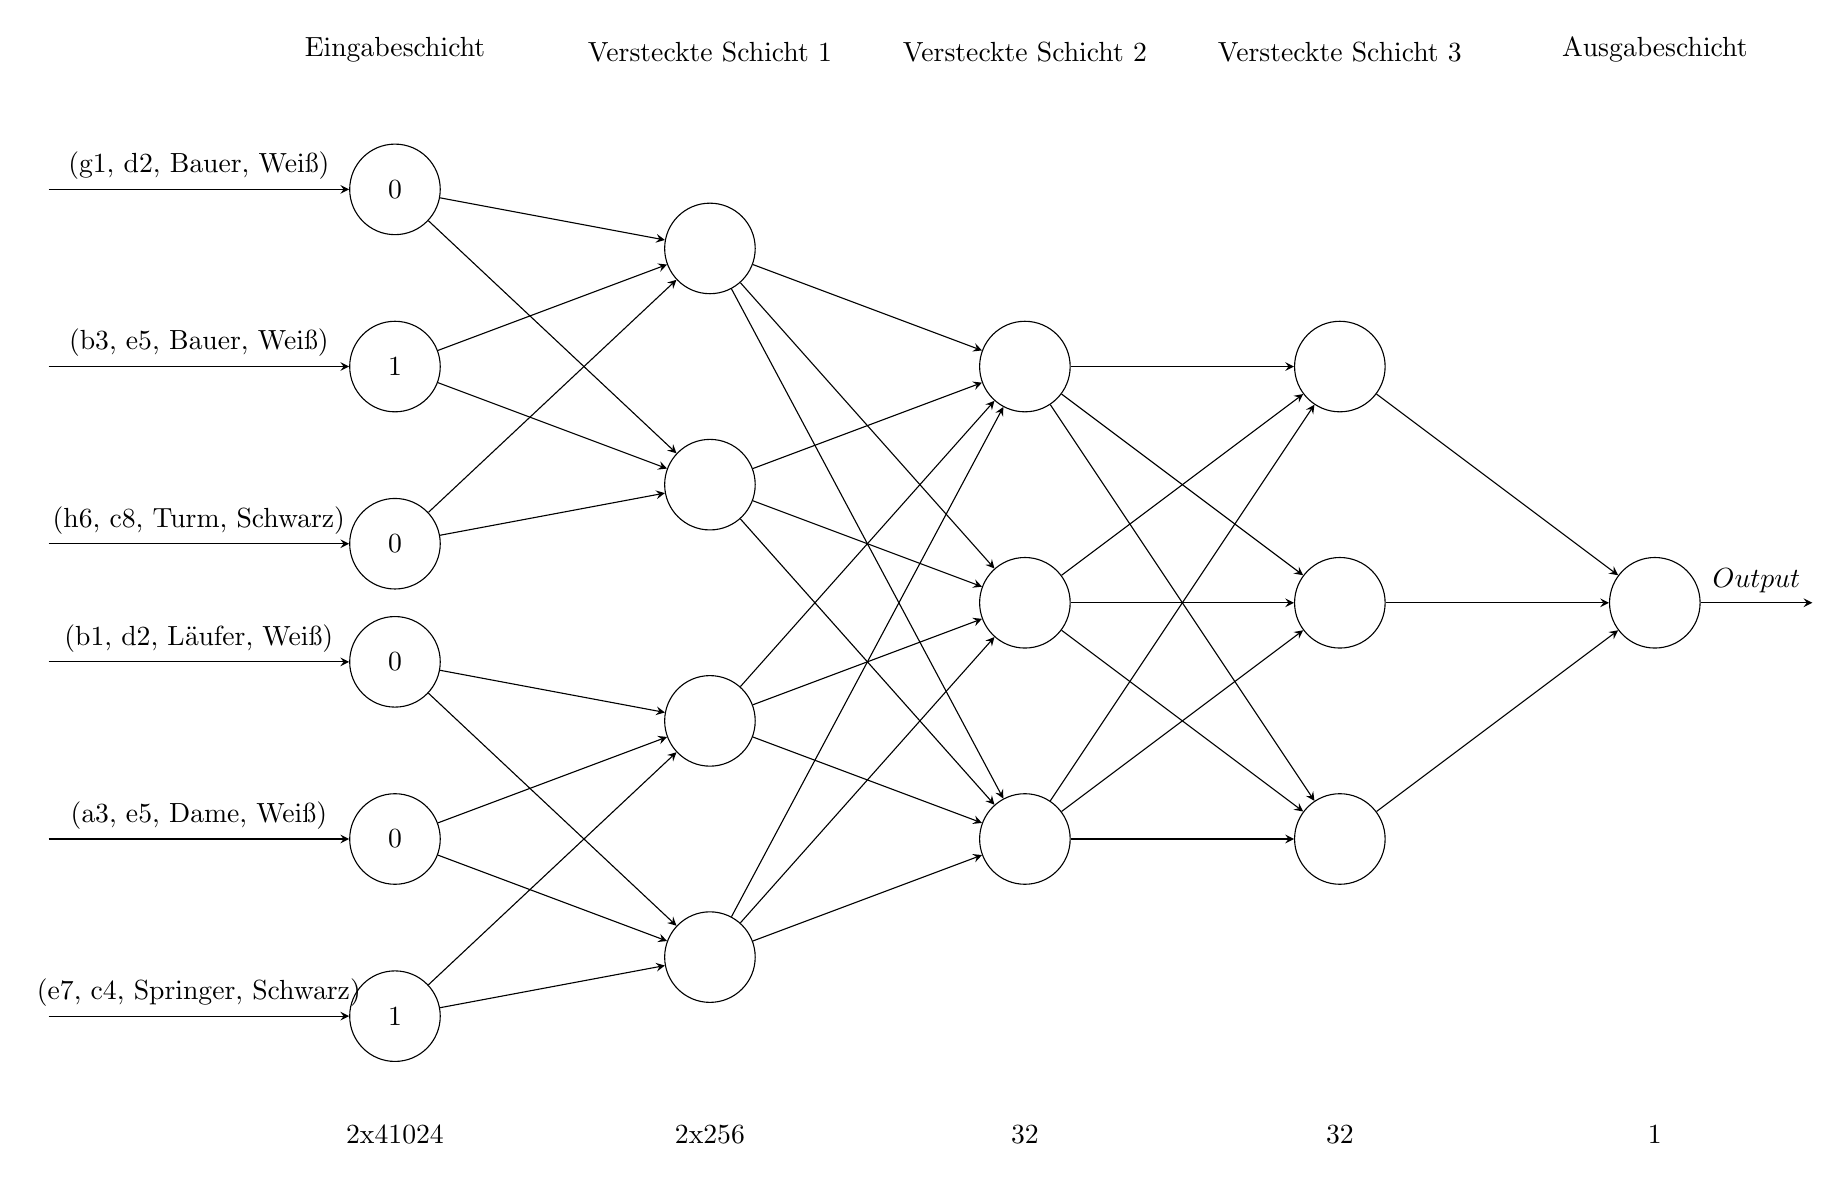
\begin{tikzpicture}[x=2cm, y=1.5cm, >=stealth]
    \tikzstyle{neuron}=[draw,shape=circle,minimum size=1.15cm]
    % draw nerons

    \foreach \m/\l [count=\y] in {0,1,0}
    \node [neuron] (input1-\y) at (0,2.5-\y*1.5) {\m};

    \foreach \m/\l [count=\y] in {0,0,1}
    \node [neuron] (input2-\y) at (0,-1.5-\y*1.5) {\m};

    \foreach \m [count=\y] in {1,2}
    \node [neuron] (inputL11-\m) at (2,2.5-\y*2) {};

    \foreach \m/\l [count=\y] in {1,2}
    \node [neuron] (inputL12-\m) at (2,-1.5-\y*2) {};

    \foreach \m/\l [count=\y] in {1,2,3}
    \node [neuron] (hidden1-\m) at (4,1.5-\y*2) {};

    \foreach \m/\l [count=\y] in {1,2,3}
    \node [neuron] (hidden2-\m) at (6,1.5-\y*2) {};

    \foreach \m [count=\y] in {1}
    \node [neuron] (output-\m) at (8,-1.5-\y) {};

    % draw text  

    \foreach \l [count=\x from 0] in {2x41024, 2x256, 32, 32, 1}
    \node [align=center] at (\x*2,-7) {\l};
  
    \draw [->] (output-1) -- ++(1,0) node [above, midway] {$Output$};

    \foreach \l [count=\x from 0] in {Eingabeschicht, Versteckte Schicht 1, Versteckte Schicht 2, Versteckte Schicht 3, Ausgabeschicht}
    \node [align=center, above] at (\x*2,2) {\l};
    % draw lines  

    \draw [->] (-2.2,1) node {} -- node [midway,above] {(g1, d2, Bauer, Weiß)} (input1-1);
    \draw [->] (-2.2,-0.5) node {} -- node [midway,above] {(b3, e5, Bauer, Weiß)} (input1-2);
    \draw [->] (-2.2,-2) node {} -- node [midway,above] {(h6, c8, Turm, Schwarz)} (input1-3);

    \draw [->] (-2.2,-3) node {} -- node [midway,above] {(b1, d2, Läufer, Weiß)} (input2-1);
    \draw [->] (-2.2,-4.5) node {} -- node [midway,above] {(a3, e5, Dame, Weiß)} (input2-2);
    \draw [->] (-2.2,-6) node {} -- node [midway,above] {(e7, c4, Springer, Schwarz)} (input2-3);

    \foreach \i in {1,2,3}
    \foreach \j in {1,2}
    \draw [->] (input1-\i) -- (inputL11-\j);
    
   \foreach \i in {1,2,3}
   \foreach \j in {1,2}
   \draw [->] (input2-\i) -- (inputL12-\j);

    \foreach \i in {1,2}
    \foreach \j in {1,2,3} {
    \draw [->] (inputL11-\i) -- (hidden1-\j);
    \draw [->] (inputL12-\i) -- (hidden1-\j);};

    \foreach \i in {1,2,3}
    \foreach \j in {1,2,3}
    \draw [->] (hidden1-\i) -- (hidden2-\j);

    \foreach \i in {1,2,3}
    \foreach \j in {1}
    \draw [->] (hidden2-\i) -- (output-\j);

  \end{tikzpicture}
  }%
  \caption{Ein einfaches \acl{NN}}
  \label{fig:own-nn}
\end{figure}

Die in dieser Arbeit verwendete Architektur ist keine neue. Sie ist die von \citeauthor{YNasu2018} \cite{YNasu2018} vorgeschlagene Architektur, die ebenfalls in der ersten \ac{NNUE} Version von Stockfish verwendet wurde.

Die Architektur ist in \autoref{fig:own-nn} zu sehen.

% the reason for choosing an architecture with two hidden layers is based on two things. 1. we dont want a large net to keep processing speed high 2. we use discoveries from other sucessfull engines that also use two hidden layers (e.g. stockfish) 
% theoratically we can use only one layer to approximate a function to convert inputs to an evaluation but thats makes it mutch harder to learn
% because we are looking for regression we use a clipped relu

Das Resultierende \ac{NN} hat 10,5 Millionen Trainierbare Parameter. Tatsächlich werden bei einer Aktivierung Maximal

% dropoutlayers are used in other chess engines and could be beneficial here

\subsection{Akkumulator}


% sparse inputs -> little changes
% max 32 inputs setboolean
% input either 0 or 1
Für den Akkumulator ist es wichtig, dass bei der Quantisierung ein Quantisierungsschema verwendet wurde, welches einen Überlauf verhindert, egal welche Kombination von Merkmalen aktiv ist \cite{StockfishNNUE}.

\subsection{Versteckte Schichten}

\subsection{Ausgabeschicht}

% the NN is a regressor becuase it only has one output note (cite?)

\section{Training}

\subsection{Eingabedaten}

Die Erzeugung der Eingabedaten ist nicht teil dieser Arbeit. Jedoch ist es wichtig zu wissen wie die Eingabedaten generiert worden und wie sie in den Trainer geladen werden, um zu verstehen, wie das neuronale Netz lernt. Im Training für diese Arbeit wurden drei verscheiden generierte Datensätze verwendet. Diese Datensätze wurden von Stockfish für das Training der neusten Variante ihres \acp{NNUE} verwendet \cite{StockfishNewestNetJul04}. Sie

% wenn eingabe daten mit einer tieferen suche verwendet werden, sind die Konzepte hinter den zügen/der evaluation schwerer zu verstehen und somit auch schwiriger zu lernen

% normalerweise ist wird pro epoche das gesamte datenset verarbeitet, hier ist das nicht der fall, wir verarbeiten 100M Positionen pro zug, wichtig ist das die daten nicht sequentiell gelesen werden, deshalb werden zufällig positionen übersprungen -> würden die daten gesuffelt sein wären die eingabedaten sehr viel größer, da ihr encoding auf sich wenig änderden positionen basiert
% Letztendlich werden alle Positionen gleichoft trainiert, die verteilung ist jedoch besser zum lernen.

% they are alerady normalized (siehe feature set)
% labeling is easy as the set is automatically generated data with labels (cp score) automatically generated

% grouping the inputdate to a batch size aims to use the time writing to the CPU more efficently (16384)

% there is no great risk of overfitting to the training set because the input data is so large -> generalisation should be strong enogth so that training data acurracy and validation data accuracy cant diverge, and becuase we dont know what the "correct" input looks like any validation data set is usless
% ein Problem ist auch das die Eingabedaten nicht wirklich den tatsächlichen anwendungsfall representieren -> das netzwerk soll die akutelle stellung gut bewerten bekommt aber als eingabe die bewertung der stelltung in zb. 5 Zügen. 

Theoretisch gibt es Daten die, \enquote{Perfekt} sind, denn Schach ist für Stellungen mit 7 Figuren gelöst. Das heißt, es gibt eine Datenbank die das eindeutige Ergebnis (-1, 0, 1) für die Position mit perfektem Spiel kennt. Es ist jedoch nicht sinnvoll diese Informationen für das Training eines \acp{NNUE} zu verwenden. Das Netz ist nicht in der Lage zu verstehen, warum die Stellung gewonnen/verloren ist. Die Konzepte sind oft schwer zu verstehen und der Vorteil wird oft erst in weiter Zukunft realisiert.

% TODO: nicht zufrieden mit dem titel
\subsection{Trainer}

% Trainer means the (pytorch lightning) module that is responsible for training

% descripe training steps:
% 1. initilize network
% repeat folloing steps for each iteration
% 2. forward activation
  % die aktivierungs funktion is eine ClippedReLU
% 3. evaluate loss either with crossentropy or mse (bouth testet, whats best is in the results chapter)
% 4. backpropagation using the Adadelta optimization algorithm
  % benefits: no learning rate tuning needed is already implemented in pytorch
\cite{Zeiler2012}

% -- epoch is an arbirairy number because we are just continiusly looping thru the data in a "shuffeling" way skipping fens not suitable for learning -> dermined by stockfish data loader

% loging with tensorboard to save results to analyze later

\section{Integration in einen Schachcomputer}

\subsection{Quantisierungsschema}

Quantisierung ist nötig, um CPU Optimierungen zu ermöglichen. Die als float trainierten Gewichte und Bias werden bei der Konvertierung des Netzes von einem \emph{.ckpt} zu einer Proprietären binären \emph{.nnue} Datei konvertiert. Alternativ kann die Konvertierung beim Einlesen der Gewichte und Bias in den Schachcomputer stattfinden. Das hat den kleinen Nachteil, dass die Netzwerkdatei etwas mehr Speicherkapazität braucht. Das hier verwendete Quantisierungsschema ist dem von Stockfish nachempfunden \cite{StockfishNNUE}. Es ist daran ausgerichtet die kleinstmöglichen Integer Typen zu verwenden. Aufgrund der Clipped \ac{ReLU} Transferfunktion sind die gewichte, bereits sehr klein, deshalb werden sie mit bestimmten Faktoren multipliziert, um eine hohe Präzision beizubehalten. Der Bereich der  In \autoref{table:netQuantization} sind die Faktoren und Datentypen für jede Schicht angegeben, die zwei versteckten Sichten unterscheiden sich nicht und werden deshalb in der Auflistung zusammengefasst. Der Ausgabetyp der Schichten ist ebenfalls aufgelistet, er ist nicht Teil der Quantisierung der Gewichte und Bias, aber wichtig für das Verständnis.

\begin{table}[h]
  \caption{Skalierfaktor und Datentypen für Gewichte und Bias des \acp{NNUE}, sowie Ausgabetyp der Schichten}
  \label{table:netQuantization}
  \renewcommand{\arraystretch}{1.2}
  \centering
  \sffamily
  \begin{footnotesize}
    \begin{tabular}{l l l l l l}
      \toprule
      \textbf{Schicht}            & \textbf{Gewicht Skalierfaktor} & \textbf{Gewichtstyp} & \textbf{Bias Skalierfaktor} & \textbf{Biastyp} & \textbf{Ausgabetyp} \\
      \midrule
      \emph{Eingabeschicht}       & 127                            & int16                & 127                         & int16            & int8                \\
      \emph{versteckte Schichten} & 64                             & int8                 & 8128                        & int32            & int8                \\
      \emph{Ausgabeschicht}       & \textasciitilde75,59           & int8                 & 9600                        & int32            & int32               \\
      \bottomrule
    \end{tabular}
  \end{footnotesize}
  \rmfamily
\end{table}

Für die Aktivierung der Schichten ändert sich der Bereich der Clipped \ac{ReLU} von 0 bis 1 zu 0 bis 127, dadurch kann der Ausgabetyp int8 sein. Der Gewichtstyp der Eingabeschicht muss int16 sein, weil er sonst bei der Akkumulation der HalfKP Features Überlaufen kann. Das Problem stellt sich, bei den versteckten Schichten nicht, da durch \ac{SIMD} Instruktionen, bei der Berechnung des Matrixprodukts der Datentyp automatisch auf int32 angepasst wird. Ein Problem, das bei den versteckten Schichten auftreten kann, ist das Überlaufen der int8 werte, deshalb werden sie vor der Multiplikation mit in beide Richtungen durch $127/64$ begrenzt. Der Bias in den versteckten Schichten und der Ausgabeschicht ist hoch, da wir sie mit den int32 Werten der Matrixprodukte addieren und maximale Präzision beibehalten. Die Ausgabeschicht besitzt einen noch höheren Bias Skalierfaktor, weil die Ausgabe der \ac{NNUE} Evaluationsfunktion der \ac{HCE} gleichen soll (für hybride Evaluation). Der Gewicht Skalierfaktor der Ausgabeschicht fällt aus der Reihe, da er nicht Ganzzahlig ist, das liegt daran, dass er sich an dem Bias Skalierfaktor und dem Aktivierungsbereich (127) anpasst, also $9600/127~=75,59$.
% warum ist der bias faktor so hoch? - Erklären

\subsection{Eingabeschicht}


\subsection{Versteckte Schicht}